%%=============================================================================
%% Appendix Code Google AutoML
%%=============================================================================

\chapter{Code Google Cloud AutoML}
\label{ch:app:google-automl}

De onderstaande code is een aangepaste versie van een algemeen script dat voor andere \textit{cloud services} binnen de \textit{vision API} gebruik kan worden. De integratie met online opslag is de makkelijkste manier om modellen te trainen, vaak worden ze in dezelfde formule aangeboden. Het code-skelet van \textcite{Guo2018} is herbruikbaar, volgende zaken moeten aangepast worden:

\begin{itemize}
    \item De namen van de mappen die de data bevat, merk op dat de namen van de mappen ook gebruikt worden om het label van elke afbeelding te bepalen
    \item Het pad naar de gebruikte \textit{bucket} op Google Cloud Storage
    \item Het formaat van de afbeeldingen
\end{itemize}

Deze stappen voldoen op voorwaarde dat volgende mappenstructuur gebruikt wordt:

\dirtree{%
    .1 online bucket.
    .2 cat.
    .3 cat.0.jpg.
    .3 cat.1.jpg.
    .3 cat.2.jpg.
    .2 dog.
    .3 dog.0.jpg.
    .3 dog.1.jpg.
    .3 dog.2.jpg.
}

Dit voorbeeld is gebruikt voor binaire classificatie maar kan zonder extra stappen (in de code) gebruikt worden voor meerdere klassen. Gewoon een nieuwe map toevoegen en dezelfde regels toepassen. Het platform zal zelf het aantal gebruikte klassen herkennen.

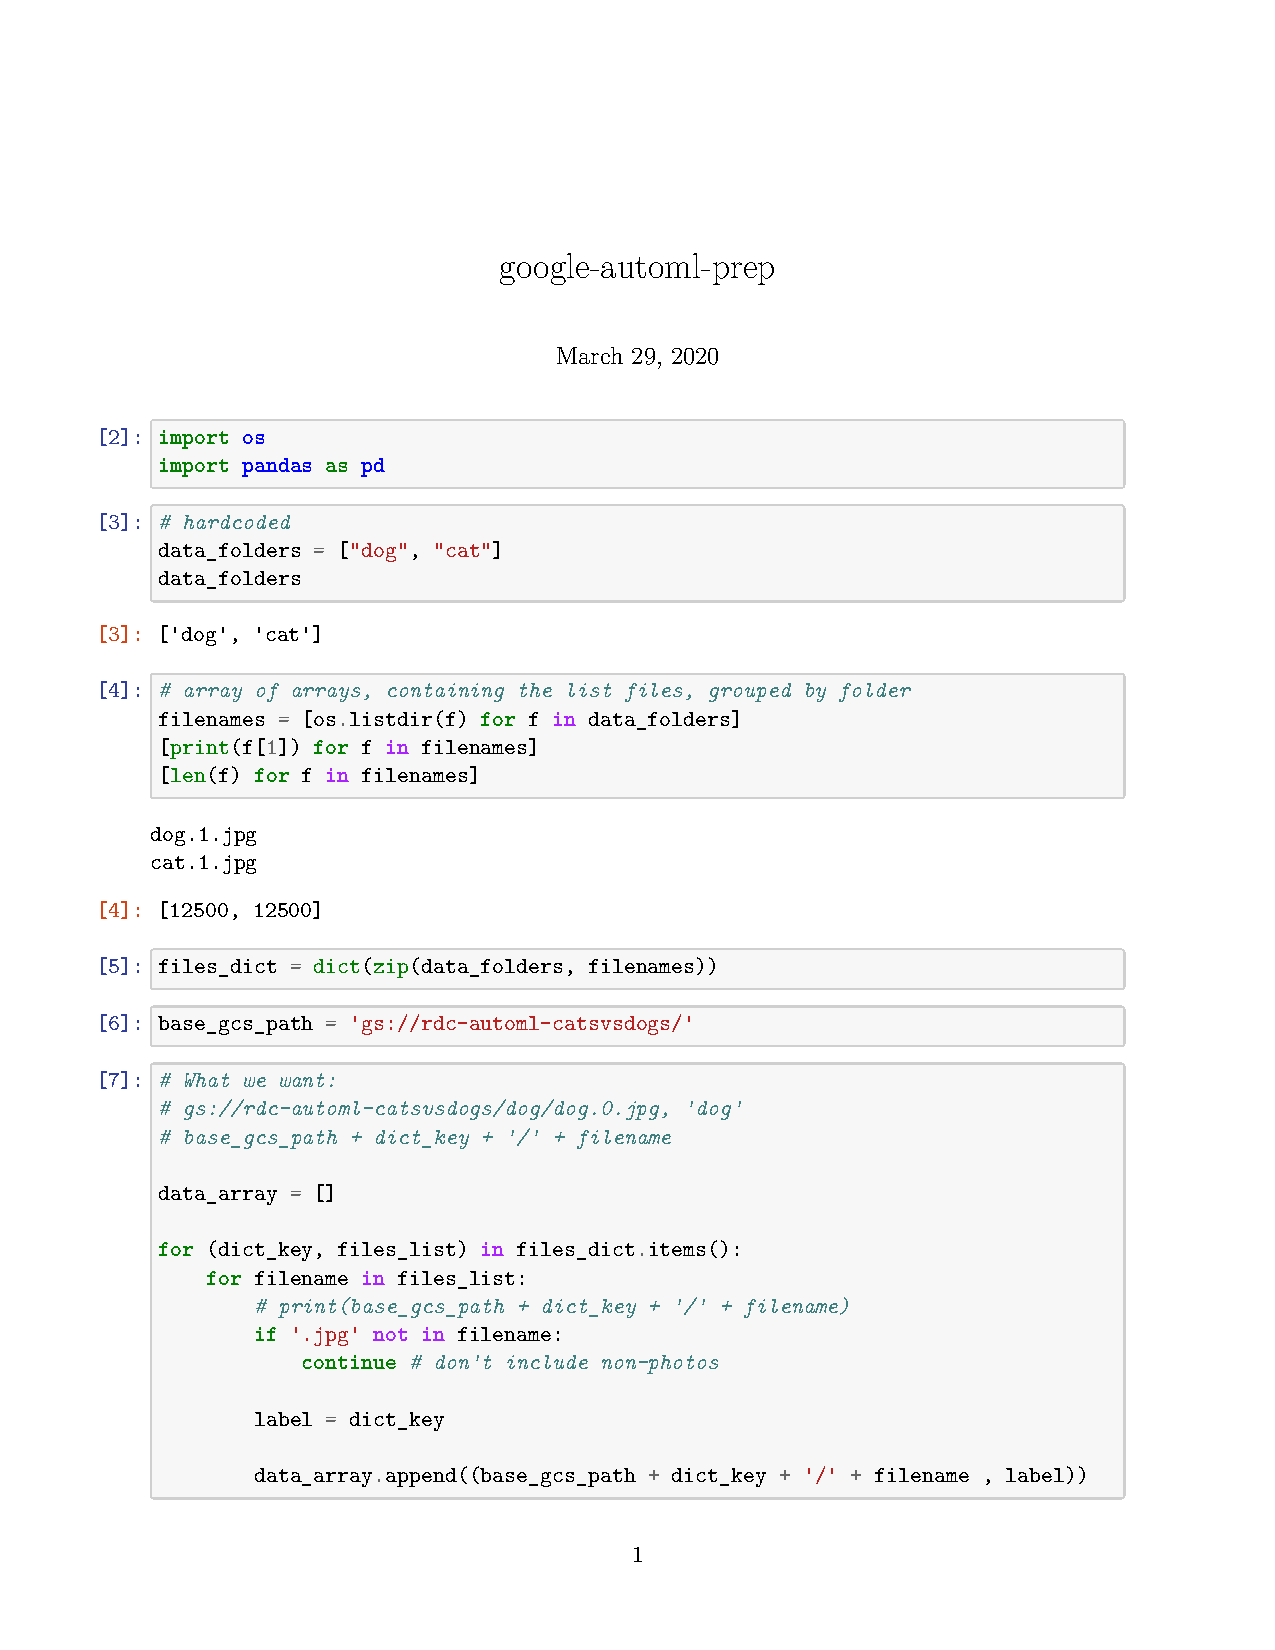
\includepdf[pages=-]{./nbconvert/google-automl-prep.pdf}